\begin{chapter}{Introduction}
\label{ch:introduction}
Various forms of noise occur in many forms of data acquisiation, transmission and processing.y
This noise needs to be removed in order to obtain a meaningful interpretation of the data, to enable further processing or, as in many image processing 
applications, just for aesthetical reasons. A common everyday example for a noisy image is taking a picture with a digital camera (e.g. integrated in a smart phone) in a weakly illuminated room:
Especially the dark areas of the picture are not uniform in color and brightness but have small variations from pixel to pixel.\\

A noise removal algorithm needs to remove these small variations but at the same time not alter important features of the data. In the case of images important features are for example 
the edges separating areas of different colors and providing the necessary sharpness of the picture. These edges on the other hand are characterized by large variations. This distinction
between small and large variations is also helpful in the task of inpainting, which tries to restore the picture at unknown or damaged regions.\\

The method of total variation(TV) noise removal, which has the above described capabilities, was first introduced by Rudin, Osher and Fatemi \cite{RudinOsher} in 1992
for the case of real-valued, that means grayscale images. Their method is briefly summarized in the following section.

\section{Grayscale images}
Let $u_0: \Omega\subset \mathbb{R}\to \mathbb{R}$ desribe the original, noise-free image, where the image domain $\Omega$ is usually a rectangular or cuboid subset of $\mathbb{R}^2$ or $\mathbb{R}^3$, respectively. 
Assuming the original pictures is corrupted by gaussian noise $n: \Omega\to\mathbb{R}$ with zero mean and variance $\sigma^2$ the noisy picture is given by $u: \Omega\to \mathbb{R}$, where
$u = u_0 + n$. The edge preserving denoising of the picture is then equivalent to the solution $u^* :\Omega\to \mathbb{R}$ of the following constrained optimization problem:
\begin{align}
    \label{osher_opt}
    u^* &= \operatorname{argmin}_{f: \Omega\to \mathbb{R}}\int_\Omega\left\vert\nabla u\right\vert  \quad\text{s.t.}\\
    \int_\Omega(u-u_0) &= 0, \quad\text{and} \int_\Omega(u-u_0)^2 = \sigma^2
\end{align}

The first term $TV(u)=\int_\Omega\left\vert\nabla u\right\vert$ is called the total variation of $u$. Rudin, Osher and Fatemi then use a partial differential equation (PDE) approach to solve
the corresponsing Euler-Lagrange equation for (\ref{osher_opt}). Later Chambolle and Lions \cite{ChambolleLions} showed that (\ref{osher_opt}) is equivalent to the minimization of
the functional
\begin{equation}
    \label{osher_func}
    \frac{1}{2}\norm{u-u_0}_2^2 +\lambda \int_\Omega\left\vert\nabla u\right\vert
\end{equation}

\subsection{Edge preservation} % (fold)
\label{sub:Edge preservation}
A basic intuition why the $L^1$ norm in (\ref{osher_func}) is besser suited for conserving sharp discontinuities such as edges can be seen from the following plot.\\

\begin{figure}[h!]
        \centering
	    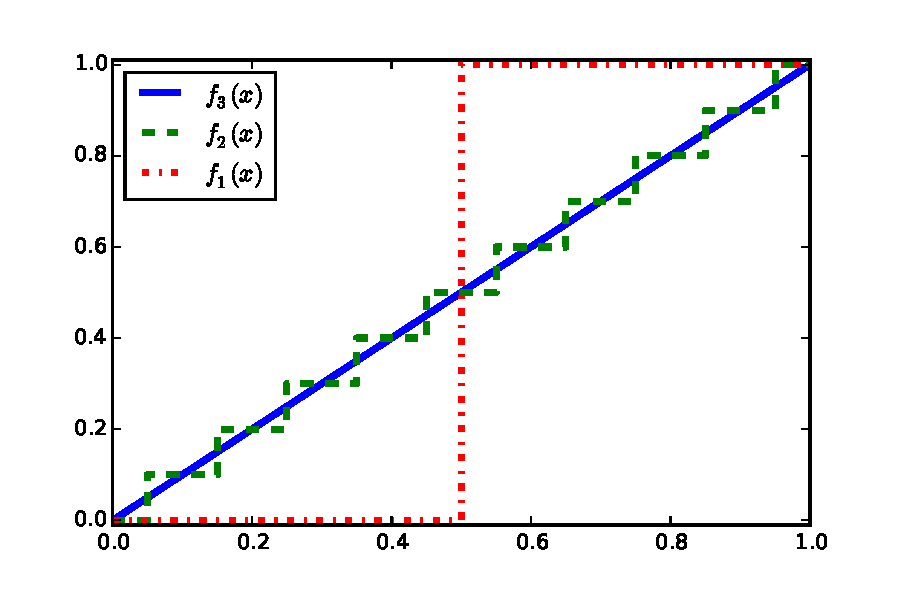
\includegraphics[width=0.9\linewidth]{./figures/introduction/tv12comparison.pdf}
	\caption[Comparison total variation]{Plots of three functions with ($N=1,\;10,\;100$) steps and a total variation equal to $1.0$}
	\label{fig:tv12comparison}
\end{figure}
\begin{table}[h!]
\centering
\begin{tabular}{|l|l|l|}
    \hline
    \textbf{Function} & $\int_{[0,1]}\left\vert\nabla f\right\vert$ & $\int_{[0,1]}\left\vert\nabla f\right\vert^2$ \\
    \hline
    $f_1$ & 1.0 & 1.0 \\
    $f_2$ & 1.0 & 0.1 \\
    $f_3$ & 1.0 & 0.01 \\
    \hline
\end{tabular}
\end{table}

One can see that the $L^2$ variation term favors continuous transitions such as $f_3$ rather than the sudden jump in $f_1$ whereas the total variation is the same for
all cases.
% subsection Edge preservation (end)

\section{Color Images}
The next step in the development of image denoising algorithms was their generalization to color images. From a mathemtical perspective this just means considering pictures
from $\Omega\to C\simeq \mathbb{R}^3$ where the form and additional properties of $C$ depend on the chosen color model. \\
In the most simple case of linear models, like RGB for instance, one could choose $C$ as $[0,1]^3$ and consider denoising each component individually (channel-by-channel model)
or consider $\mathbb{R}^3$ as a normed vector space of tuples $(x_R, x_G, x_B)$ (linear-vectorial model).\\
For the nonlinear models, especially the so-called chromaticity-brightness model, Chang and Kang \cite{ChangKuang} showed the closest resemblance to human perception.
In this case we can take $C=S^2\times [0,1]$ such that the chromatictiy takes values on the sphere $S^2$ considered as a submanifold of the euclidian space $\mathbb{R}^3$, 
while the brightness is real-valued, as in the case of graysale images.

\section{Manifold-valued Images} % (fold)
\label{sec:Manifold-valued Images}
In the last section we have already seen that, depending on the chosen color model, pixels can take their values on a manifold and are usually represented by their matrices.
This data arises in a variety of application such as Diffusion Tensor Magnetic Resonance Imaging (DTI-MRI), computer vision and robotics to name just a few.

\section{Objective and Outline of this work}
In this work we will introduce an extendable multi-threaded C++ template library for the purpose of TV Minimization of manifold-valued images. 
So far the implemented minimization algorithms are based on the iteratively reweighted least squares (IRLS) adaption suggested by Sprecher and Grohs \cite{SprecherIRLS} as well as a 
proximal point algorithm by Weinmann et al \cite{WeinmannPRPT}. We extend the implementation to 3D images cubes, the Grassmann manifold and also provides some quasi-analytic expressions
for derivatives of the Riemannian distance function.\\

In the following chapter 2 a short summary of the necessary theory, a description of the algorithms and relevant properties for each of the implemented manifolds.
After that the chapter 3 introduces the library itself in particular its capabilieties, design concepts, structure, installation and usage in the form of some typical
use cases. In Chapter 4 numerical experiments are conducted, showing various application of the library as well as convergence behavior and comparisons between 
IRLS and proximal point based minimizers.\\

Finally, chapter 5 concludes with possible extensions and adaptions of the library, in particular possibility of recursive splitting of the image domain into smaller subproblems and
the transition to distributed architectures.
% section Manifold-valued Images (end)
\end{chapter}
